
\documentclass[../../../all/physics-standard_questions_all.tex]{subfiles}

\graphicspath{{../../../../figures/}}

\begin{document}

\begin{enumerate}

    \item 図のように，電池E（起電力$V_0$），電気抵抗R$_1$（抵抗値$2R$），
        R$_2$（抵抗値$3R$）からなる回路がある．R$_2$の電位差（電圧）$V_2$を求めよ．
        %
        \par \vspace{0.2\baselineskip}
        {\centering
            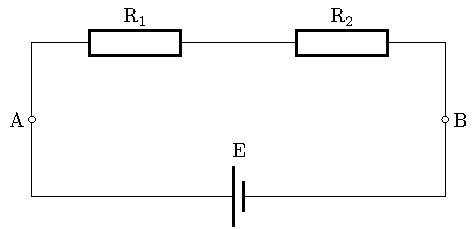
\includegraphics{q_circuit-basics_01_01/physics-standard_questions_circuit-basics_01_01_tikz.pdf}
        \par}
        \vspace{0.2\baselineskip}

    \item 図のように，電池E（起電力$V_0$），電気抵抗R$_1$（抵抗値$2R$），R$_2$（抵抗値$R$），
        R$_3$（抵抗値$2R$）からなる回路がある．
        R$_2$を流れる電流の大きさ$i$を求めよ．
        %
        \par \vspace{0.2\baselineskip}
         {\centering
            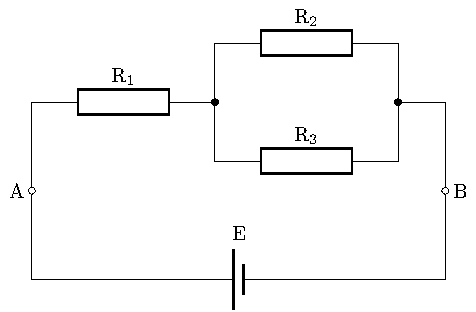
\includegraphics{q_circuit-basics_01_02/physics-standard_questions_circuit-basics_01_02_tikz.pdf}
        \par}
        \vspace{0.2\baselineskip}

    \item 図のように，電池E$_1$（起電力$2V_0$），E$_2$（起電力$V_0$），
        電気抵抗R$_1$（抵抗値$R$），R$_2$（抵抗値$R$），R$_3$（抵抗値$2R$）からなる回路がある．
        AB間を流れる電流の大きさ$I$を求めよ．
        %
        \par \vspace{0.2\baselineskip}
        {\centering
            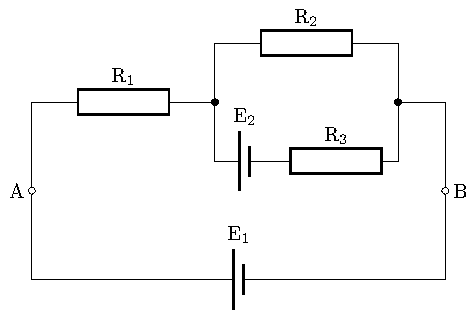
\includegraphics{q_circuit-basics_01_03/physics-standard_questions_circuit-basics_01_03_tikz.pdf}
        \par}
        \vspace{0.2\baselineskip}

    \item \needspace{10\baselineskip} 
        図のように，電池E（起電力$V_0$），電気抵抗R$_1$（抵抗値$2R$），R$_2$（抵抗値$R$），
        R$_3$（抵抗値$R$），R$_4$（抵抗値$R$），R$_5$（抵抗値$R$）からなる回路がある．
        AB間を流れる電流の大きさ$I$を求めよ．
        %
        \par \vspace{0.2\baselineskip}
        {\centering
            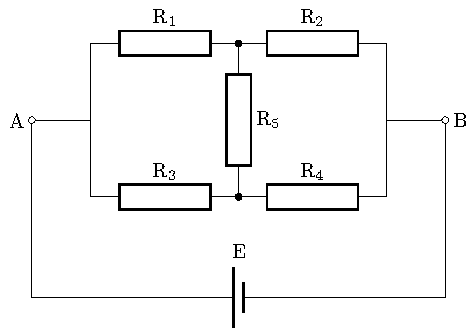
\includegraphics{q_circuit-basics_01_04/physics-standard_questions_circuit-basics_01_04_tikz.pdf}
        \par}
        \vspace{0.2\baselineskip}

\end{enumerate}

\end{document}
